\let\negmedspace\undefined
\let\negthickspace\undefined
\documentclass[journal]{IEEEtran}
\usepackage[a5paper, margin=10mm, onecolumn]{geometry}
%\usepackage{lmodern} % Ensure lmodern is loaded for pdflatex
\usepackage{tfrupee} % Include tfrupee package

\setlength{\headheight}{1cm} % Set the height of the header box
\setlength{\headsep}{0mm}     % Set the distance between the header box and the top of the text

\usepackage{gvv-book}
\usepackage{gvv}
\usepackage{cite}
\usepackage{amsmath,amssymb,amsfonts,amsthm}
\usepackage{algorithmic}
\usepackage{graphicx}
\usepackage{textcomp}
\usepackage{xcolor}
\usepackage{txfonts}
\usepackage{listings}
\usepackage{enumitem}
\usepackage{mathtools}
\usepackage{gensymb}
\usepackage{comment}
\usepackage[breaklinks=true]{hyperref}
\usepackage{tkz-euclide} 
\usepackage{listings}
% \usepackage{gvv}                                        
\def\inputGnumericTable{}                                 
\usepackage[latin1]{inputenc}                                
\usepackage{color}                                            
\usepackage{array}                                            
\usepackage{longtable}                                       
\usepackage{calc}                                             
\usepackage{multirow}                                         
\usepackage{hhline}                                           
\usepackage{ifthen}                                           
\usepackage{lscape}
\begin{document}

\bibliographystyle{IEEEtran}
\vspace{3cm}

\title{1-1.5-1}
\author{EE24BTECH11060 - Sruthi Bijili}
% \maketitle
% \newpage
% \bigskip
{\let\newpage\relax\maketitle}

\renewcommand{\thefigure}{\theenumi}
\renewcommand{\thetable}{\theenumi}
\setlength{\intextsep}{10pt} % Space between text and floats


\numberwithin{equation}{enumi}
\numberwithin{figure}{enumi}
\renewcommand{\thetable}{\theenumi}

\textbf{Question}:\\
The centre of the circle whose end points of the diameter are \brak{-6, 3} and \brak{6, 4} is \\


\hfill(10, 2020)
\\
\textbf{solution:}
\begin{table}[h!]    
  \centering
  \begin{tabular}[12pt]{ |c| c|c|}
    \hline
        \textbf{Variable} & \textbf{Description} & \textbf{formula}\\
    \hline
        $\vec{A}\brak{-6,3}$ & One end of the Diameter & $-$ \\
    \hline 
        $\vec{B} \brak{6,4}$ & other end of the Diameter & $-$\\
    \hline
        $\vec{C}$& center of the circle & $-$\\ 
    \hline
        $k$ & ratio in which $\vec{c}$ divides the diameter $AB$ & $\frac{\vec{B}+k\vec{A}}{k+1}$\\
    \hline       
\end{tabular}


  \caption{Input parameters}
\end{table}
\begin{align}
k&=1\\
\implies \Vec{C}&=\frac{\Vec{A}+\Vec{B}}{2}\\
\implies \Vec{C}&=\frac{\myvec{-6 \\ 3}+\myvec{6 \\ 4}}{2}\\
\implies \Vec{C}&=\myvec{0 \\ \frac{7}{2}}
\end{align}
\begin{figure}[h!]
   \centering
   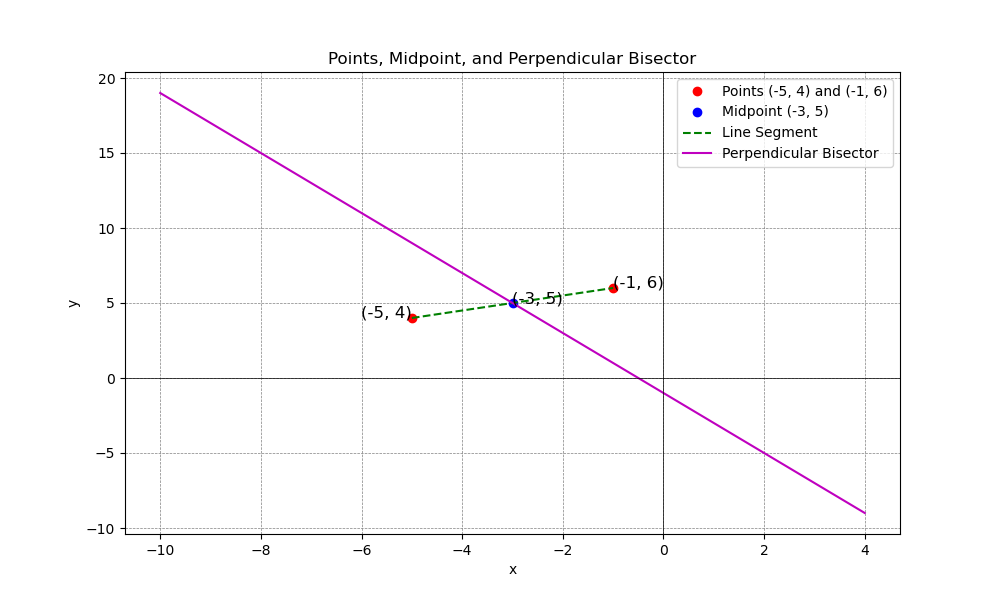
\includegraphics[width=0.7\linewidth]{figs/fig1.png}
   \caption{circle with diameter AB}
\end{figure}


    





\end{document}

